\section{Shor’s Algorithmus: Funktionsweise und mathematische Grundlage}
\label{sec:shor}

Shor’s Algorithmus ist ein Quantenalgorithmus, der entwickelt wurde, um 
effizient die Primfaktoren einer großen Zahl $N$ zu bestimmen. Dieses 
Problem bildet die Grundlage vieler kryptografischer Verfahren wie RSA, 
da es für klassische Computer äußerst schwierig ist, große Zahlen in 
ihre Primfaktoren zu zerlegen. Shor’s Algorithmus hingegen nutzt die 
Eigenschaften von Quantencomputern, um diese Aufgabe exponentiell 
schneller zu lösen. \cite{shor}

\subsection{Ablauf des Algorithmus}

\begin{enumerate}
    \item \textbf{Auswahl einer Basis $a$:}  
    Zunächst wird eine Zahl $a$ gewählt, wobei $1 < a < N$ gilt. Diese 
    Basis dient als Ausgangspunkt für die nachfolgenden Berechnungen.

    \item \textbf{Periodenfindung:}  
    Der Algorithmus sucht die kleinste positive Periode $r$, sodass die 
    Kongruenzgleichung  
    \[
    a^r \mod N = 1
    \]  
    erfüllt ist. Die Periode $r$ ist der Schlüssel zur Faktorisierung von $N$.  
    \begin{itemize}
        \item Es wird sichergestellt, dass $r > 0$ ist, da eine Periode von 
        $r = 0$ keine Aussagekraft hat.
        \item Zur Bestimmung von $r$ könnte man klassisch eine Wertetabelle 
        für $r$ und die entsprechenden Werte $z = a^r \mod N$ erstellen. Da 
        diese Methode jedoch ineffizient ist, wird auf einem Quantencomputer 
        die \hyperref[sec:QFT]{Quanten-Fourier-Transformation (QFT)} verwendet, um $r$ effizient 
        zu berechnen.
    \end{itemize}

    \item \textbf{Verwendung der Periode $r$:}  
    Sobald $r$ bekannt ist, wird geprüft:  
    \begin{itemize}
        \item Falls $r$ ungerade ist, beginnt der Algorithmus erneut mit 
        einem anderen $a$.
        \item Ist $r$ gerade, werden die Primfaktoren von $N$ mit den 
        folgenden Formeln berechnet:  
        \[
        f_1 = \text{ggT}\left(a^{r/2} - 1, N\right) \quad \text{und} \quad f_2 = \text{ggT}\left(a^{r/2} + 1, N\right).
        \]  
        Der größte gemeinsame Teiler ($\text{ggT}$) wird dabei mithilfe 
        des Euklidischen Algorithmus ermittelt. \cite{shor_klassisch} \cite{shor_klassisch2} 
    \end{itemize}
\end{enumerate}

\subsection{Euklidischer Algorithmus: Beispiel zur Bestimmung des ggT}

Der Euklidische Algorithmus wird verwendet, um den größten gemeinsamen 
Teiler (ggT) zweier Zahlen effizient zu bestimmen. Anhand des Beispiels 
$N_1 = 132$ und $N_2 = 28$ wird der Algorithmus wie folgt angewendet:

\begin{enumerate}
    \item \textbf{Schritt 1:}  
    Teile die größere Zahl durch die kleinere und bestimme den Rest:  
    \[
    132 \div 28 = 4 \, \text{Rest} \, 20 \quad \Rightarrow \quad 132 = 4 \cdot 28 + 20.
    \]

    \item \textbf{Schritt 2:}  
    Die vorherige Divisorzahl $28$ wird der neue Dividend, und der Rest $20$ wird der neue Divisor:  
    \[
    28 \div 20 = 1 \, \text{Rest} \, 8 \quad \Rightarrow \quad 28 = 1 \cdot 20 + 8.
    \]

    \item \textbf{Schritt 3:}  
    Wiederhole den Vorgang, bis der Rest $0$ wird:  
    \[
    20 \div 8 = 2 \, \text{Rest} \, 4 \quad \Rightarrow \quad 20 = 2 \cdot 8 + 4,
    \]  
    \[
    8 \div 4 = 2 \, \text{Rest} \, 0 \quad \Rightarrow \quad 8 = 2 \cdot 4 + 0.
    \]
\end{enumerate}

Der letzte Divisor, bevor der Rest $0$ wird, ist der gesuchte größte gemeinsame Teiler: \cite{euklid}
\[
\text{ggT}(132, 28) = 4. 
\] 

Im Hinblick auf unsere Forschungsfrage lässt sich festhalten, dass Shor's Algorithmus eine 
Methode darstellt, mit der die Berechnung eines kryptografischen Schlüssels effektiv rückgängig 
gemacht werden kann. Die Sicherheit vieler aktueller Verschlüsselungsverfahren, wie RSA, basiert 
auf der Schwierigkeit, eine große Zahl in ihre Primfaktoren zu zerlegen. Shor's Algorithmus macht 
es jedoch möglich, diese beiden Primfaktoren effizient zu bestimmen, sofern ein ausreichend 
leistungsfähiger Quantencomputer zur Verfügung steht. Dadurch wird das Fundament der zugrunde 
liegenden Verschlüsselung geschwächt, da die ursprüngliche Annahme, dass die Faktorisierung ein 
praktisch unlösbares Problem sei, durchbrochen wird.

\subsection{Fourier-Transformation: Zerlegung von Signalen in Frequenzen}
Die Fourier-Transformation ist ein Algorithmus, mit einer Komplexität von \(O\left(n^2\right) \), der häufig genutzt wird, um ein Signal in ein Spektrum von Frequenzen zu zerlegen, also in eine kontinuierliche Menge an Gewichten, sodass die kontinuierliche, gewichtete Summe aus Sinus und Kosinus Funktionen unterschiedlicher Frequenzen ist. Die am häufigsten genutzte Variante ist die diskrete Fourier-Transformation, die nicht kontinuierlich ist und somit nur endliche Frequenzen erkennt. %\cite{don_h_johnson_58_2017}

\subsubsection{\textbf{Diskrete Fourier-Transformation: DFT}}\label{sec:DFT}~\newline
DFT operiert an einer diskreten Folge an komplexen Zahlen

\(a = (a_0,\dots,a_{N-1}) \in \mathbb{C}^N\) (\(a_k \in \mathbb{C}\)) und gibt eine Folge\\
\(\hat{a} = (\hat{a}_0,\dots,\hat{a}_{N-1}) \in \mathbb{C}^N\) (genannt \anf{diskret Fourier-Transformierte})
wobei \[\hat{a}_k = \sum_{j=0}^{N-1}e^{-2\pi \imath\cdot\frac{jk}{N}}\cdot a_j \quad \text{für}\quad k = 0,\dots,N-1\] oder als Matrix-Vektor-Produkt: %\cite{wiki_discrete_fourier_transformation}
\[\hat{a} = W\cdot a \quad \text{mit} \quad W[k,j] = e^{-2\pi \imath \cdot\frac{jk}{N}}\]

\subsubsection{\textbf{Interpretation der Fourier-Transformation:}}
\begin{itemize}
	\item \textbf{Bedeutung des Ergebnisses:}\\
	Mit den diskret Fourier-Transformierten lässt sich eine Funktion konstruieren, die an den stellen \(n = 0,\dots,N-1\) die originalen Funktionswerte liefert.
	\[f[n] = \sum_{k=0}^{N-1}\left(\text{Re}(\hat{a}^\prime_k)\cos\left(\frac{2\pi kn}{N}\right)+\text{Im}(\hat{a}^\prime_k)\sin\left(\frac{2\pi kn}{N}\right)\right)\]
	wobei \(\hat{a}\) zur Vereinfachung und besseren Relation normiert wird mit \(\hat{a}^\prime = \frac{\hat{a}}{N}\).
	\(f[n]\) ist eine Summe von Kosinus- und Sinusfunktionen mit einer Frequenz von \(2\pi\cdot\frac{k}{N}\), wobei für jeden Wert \(\hat{a}^\prime_k\) der Realteil Koeffizient der jeweiligen Kosinusfunktion und der negative Imaginärteil Koeffizient der jeweiligen Sinusfunktion ist.
	Eine alternative Interpretation der Werte der diskret Fourier-Transformierten ist, das \(\left\lvert \hat{a}^\prime_k\right\rvert \) der Amplitude und die Phase \(\quad\arg(\hat{a}^\prime_k) = \arctan\left(\frac{\text{Im}(\hat{a}^\prime_k)}{\text{Re}(\hat{a}^\prime_k)}\right)\quad \) entspricht.
	\[f[n] = \sum_{k=0}^{N-1}\left\lvert\hat{a}^\prime_k\right\rvert\cdot\cos\left(\frac{2\pi kn}{N}+\arg(\hat{a}^\prime_k)\right)\]
	Dies ist eine Zerlegung der Eingangssequenz in Frequenzen.
	\item \textbf{Alternative Berechnung der diskreten Fourier Transformation:}\\
	Eine menschenfreundlichere Methode kann man erhalten, wenn man erhalten, indem man die Eulersche Formel anwendet:
	\[e^{-2\pi \imath \cdot\frac{jk}{N}} = \cos\left(\frac{2\pi jk}{N}\right) + \imath\cdot\sin\left(\frac{2\pi jk}{N}\right)\]
	Nach dieser Umstellung lässt sich folgender Algorithmus herleiten:
	\begin{enumerate}
		\item \textbf{Vergleichsfunktion definieren:}\\%Assymetrische Klammern in diesen Teil sind, weil sie Intervalle sind
		Der Algorithmus funktioniert, indem man die gegebene Sequenz mit Sinus- und Cosinuskurven von verschiedenen Frequenzen vergleicht. Da der Cosinus den Real- und der Sinus den Imaginärteil stellt und diese sich nicht gegenseitig beeinflussen, wenn \(a \in \mathbb{R}^N\), kann man diese auch getrennt beachten.
		\[f_k(x) = \cos\left(\frac{2\pi k}{N}\cdot x\right) + \imath \cdot\sin\left(\frac{2\pi k}{N}\cdot x\right) \]
		Die Winkelfunktionen sollen im Intervall \([0,N)\), also im Intervall der Eingangssequenz, \(k\) ganze Perioden durchlaufen. Der Cosinus (Sinus ist analog) durchläuft eine Periode im Intervall \([0,2\pi)\). Wenn man das Argument \(x\) mit \(2\pi\), multipliziert wird das Periodenintervall zu \([0,1)\). Durch Division mit \(N\) wird das Intervall zum verlangten \([0,N)\). Um \(k\) Perioden im Intervall zu erhalten, Multipliziert man mit \(k\), sodass das Intervall \(\left[0,\frac{N}{k}\right) ~k\)-mal in \([0,N)\) passt.
		\item \textbf{Vergleichssequenzen erstellen:}\\
		Mit der Funktion können wir die \(k\)-te Vergleichssequenz erhalten, indem wir \(f\) an denselben Stellen wie \(a\) abtasten.
		\[b_k = \left(f_k(0),f_k(1),\dots,f_k(N-1)\right) \]
		\item \textbf{Vergleichen:}\\
		Um zu erfahren, welchen Teil die \(k\)-te Frequenz in der Eingangssequenz spielt, nimmt man die Summe der Produkte von jedem Element \(a_j\) der Eingangssequenz mit den korrespondierenden \({(b_k)}_j\), d.h. das Skalarprodukt
		\[\hat{a}_k = a \cdot b_k\]
		\item \textbf{Spezialfall \(k = 0\):}\\
		Schon in der Ausgangsformel kann man sehen, das	für \(k = 0\) gilt: \[e^{-2\pi \imath \cdot\frac{j\cdot 0}{N}} = e^0 = 1\]
		weshalb sich \(\hat{a}_0\) zu
		\[\hat{a}_0 = \sum_{j=0}^{N-1} a_j\] zusammenfassen lässt. Womit \(\hat{a}^\prime_0 \) dem arithmetischen Mittel von \(a\) entspricht.
	\end{enumerate}
 	%Python algo
	%j aj âj
	%0 1  9 + 0j
	%1 2  0 + 0j
	%2 1  0 + 0j
	%3 2 -3 + 0j
	%4 1  0 + 0j
	%5 2  0 + 0j
	%import numpy as np
	%a = np.array([1,2,1,2,1,2])
	%ao = [0,0,0,0,0,0]
	%ao[0] = sum(a)#O(n)
	%for i in range(1,6):#O(n*z)
	%	#z = 3*O(n) = O(n)
	%	test = np.arange(0,2*np.pi*i,2*np.pi*i/6)#O(n)
	%	ao[i] = a.dot(np.cos(test))#O(n)
	%	ao[i] += 1j*a.dot(np.sin(test))#O(n)
	%#O(n²)
	%for n in ao:
	%	print(np.round(n,5))
\end{itemize}%\cite{yt_reducible}
\subsubsection{\textbf{Quanten-Fourier-Transformation: QFT}}\label{sec:QFT}~\newline
QFT ist die Anwendung von \hyperref[sec:DFT]{DFT} in auf Quantencomputern. Sie hat \(n\) Qubits als Eingang, womit die Eingangssequenz aus \(N = 2^n\) Basiszuständen besteht: \(\left(|0\rangle,|1\rangle,\dots,|N-1\rangle\right)\). Der Quantenschaltkreis ist in Abbildung~\ref{fig:QFT_n_Qubits} zu sehen.
\begin{figure}[hb]
	\centering
	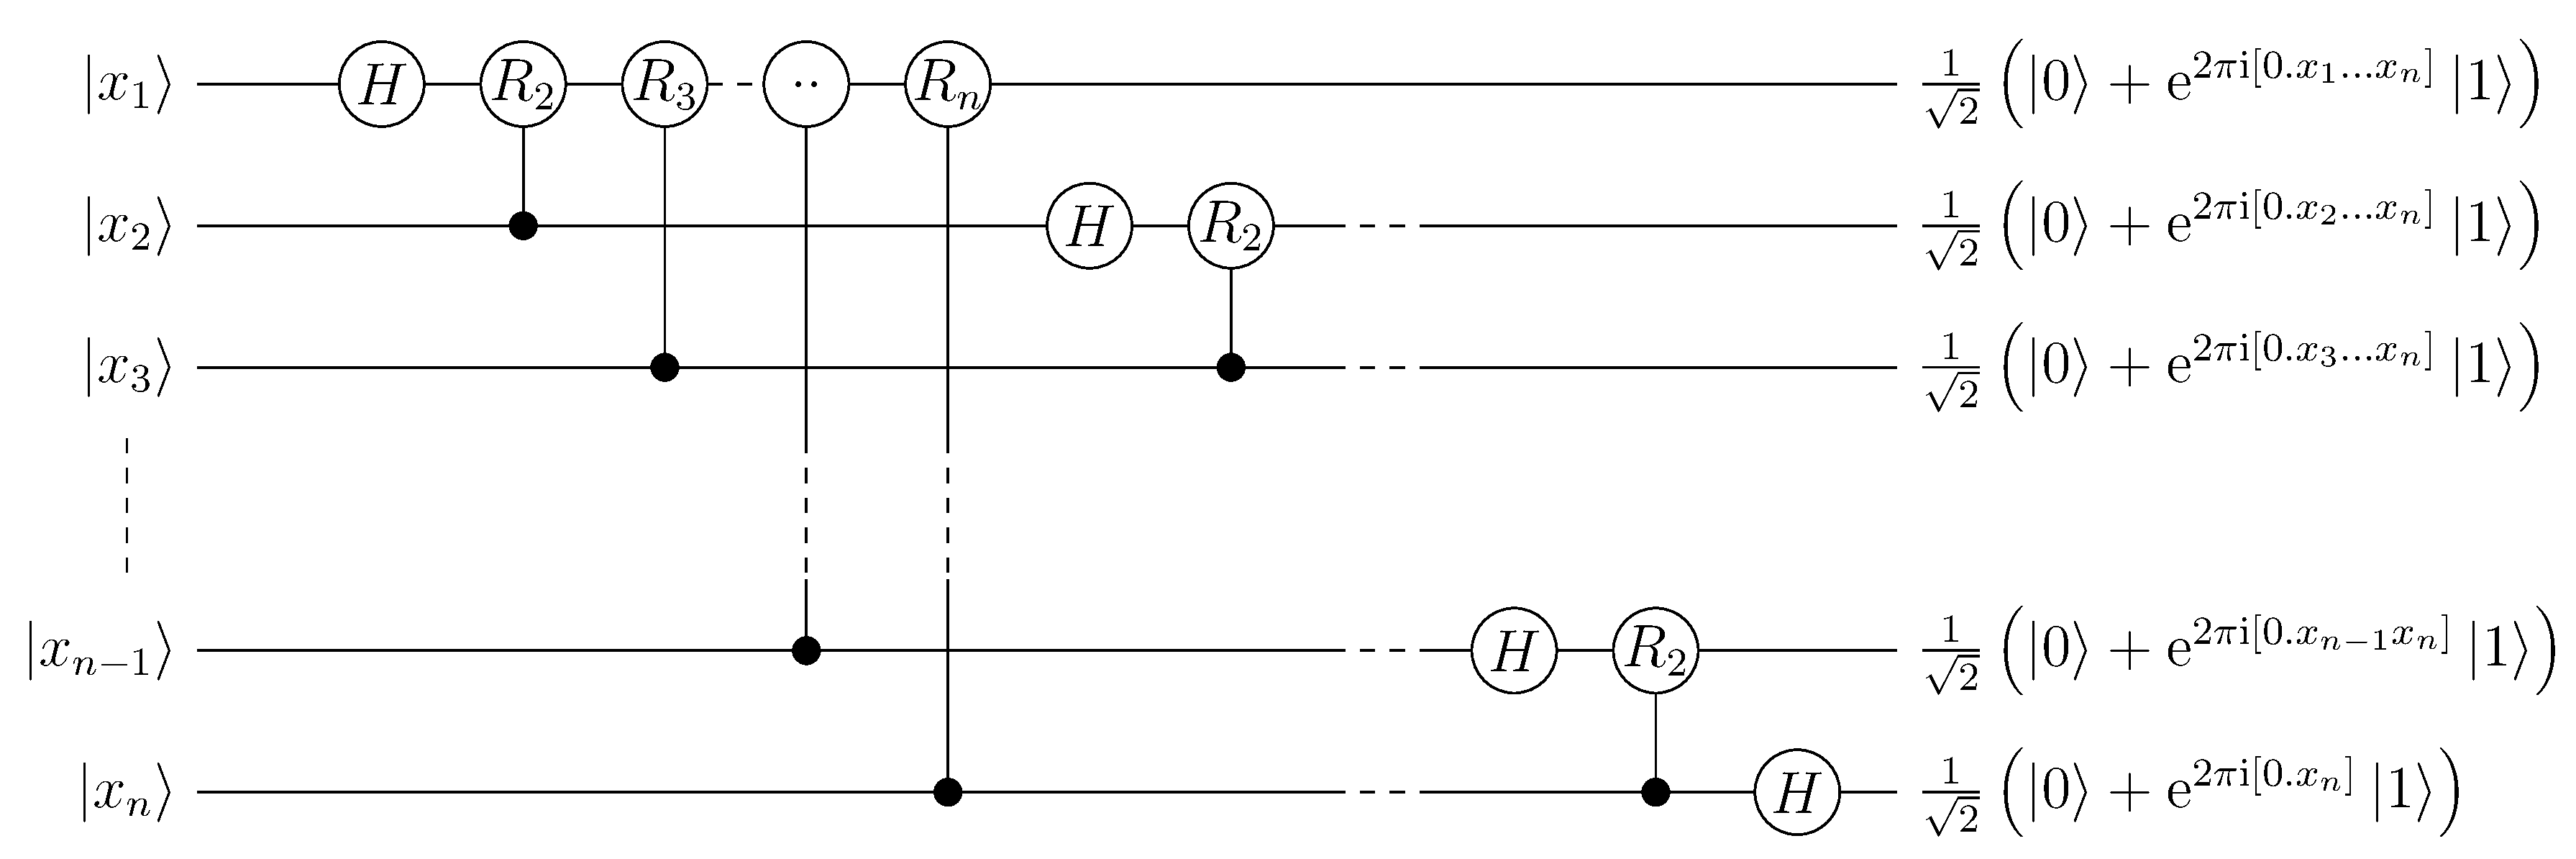
\includegraphics[width=0.45\textwidth]{sections/felix/Q_fourier_nqubits.png}
	\caption{QFT für n Qubits (ohne Umkehrung der Reihenfolge der Zustände der Ausgaben)}
	%\cite{wiki_q_fourier_nqubitspng} % in \caption einfügen nach )
	\label{fig:QFT_n_Qubits}
\end{figure}
\\Wobei \(\left[0.x_1 x_2 \dots x_n\right]\) Notation für \(\frac{x_1}{2}+\frac{x_2}{4}+\cdots+\frac{x_n}{2^n}\) ist.
Verwendet werden das Hadamard-Gatter \(H = \frac{1}{\sqrt{2}}\begin{pmatrix}
	1 &  1\\
	1 & -1
\end{pmatrix}\) und Kontrollierte Phasengatter \(R_m = \begin{pmatrix}
	1 & 0\\
	0 & e^{\frac{2\pi\imath}{2^m}}\\
\end{pmatrix}\).
Eine Schaltung für \(3\) Qubits und somit \(2^3 = 8 = N\) ist in Abbildung~\ref{fig:QFT_3_Qubits} zu sehen.%\cite{wiki_list_quantum_gates}
\begin{figure}[hb]
	\centering
	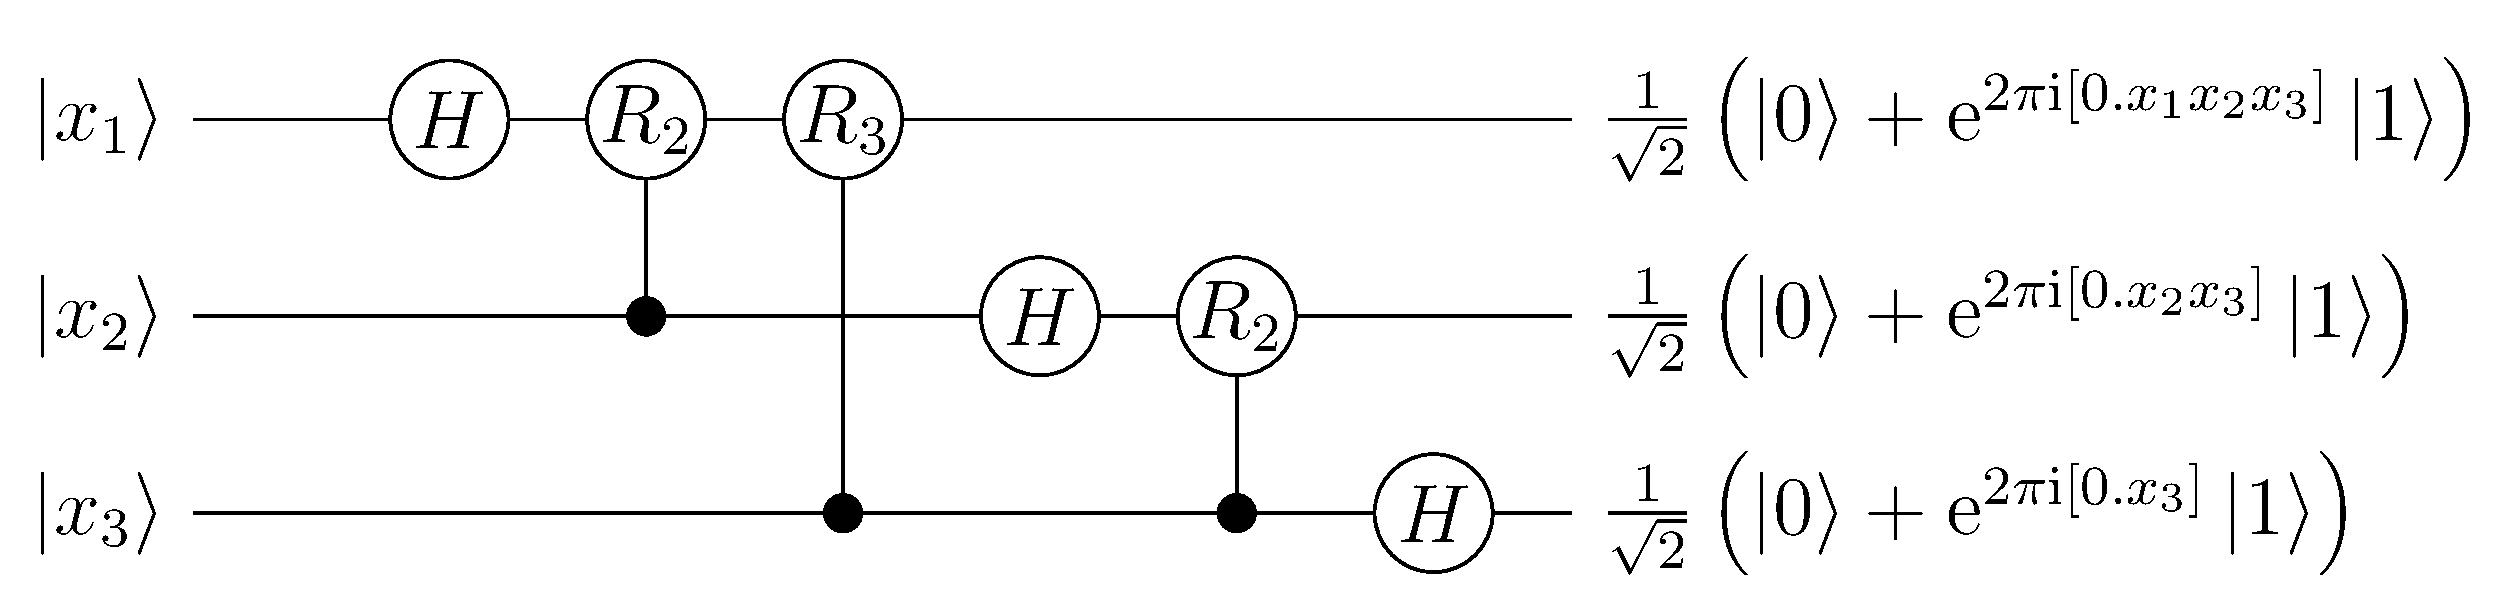
\includegraphics[width=0.45\textwidth]{sections/felix/Q_fourier_3qubits.png}
	\caption{QFT für 3 Qubits (ohne Umkehrung der Reihenfolge der Zustände der Ausgaben)}
	%\cite{wiki_q_fourier_3qubitspng} % in \caption einfügen nach )
	\label{fig:QFT_3_Qubits}
\end{figure}
\\Diese Schaltung lässt sich mithilfe der Identitätsmatrix \(I = \begin{pmatrix}
	1 & 0 \\
	0 & 1 
\end{pmatrix}\) und der Tauschmatrix \(S = \begin{pmatrix}
	1 & 0 & 0 & 0\\
	0 & 0 & 1 & 0\\
	0 & 1 & 0 & 0\\
	0 & 0 & 0 & 1
\end{pmatrix}\) in der Gleichung
\begin{multline}
	W = (S\oplus I)\cdot (I \oplus H \oplus I) \cdot (R_2 \oplus I) \cdot (I \oplus S) \cdot (I\oplus R_3)\\ \cdot (S \oplus I) \cdot (I \oplus H \oplus I) \cdot (R_2 \oplus I) \cdot (H \oplus I \oplus I)
\end{multline}
\[QFT_8 |x\rangle = W \cdot \left(|x_1\rangle \oplus |x_2\rangle \oplus |x_3\rangle\right)\]
\[\text{oder auch als}\quad QFT_8 |x\rangle = \frac{1}{\sqrt{8}}\sum_{j=0}^{8-1} e^{\frac{2\pi \imath x j}{8}}|j\rangle\]
darstellen, sodass für ein allgemeines \(N = 2^n\) gilt:
\[QFT_N |x\rangle = \frac{1}{\sqrt{N}}\sum_{j=0}^{N-1} e^{\frac{2\pi \imath x j}{N}}|j\rangle\]
%\cite{wiki_quanten-fouriertransformation}
Dies unterscheidet sich von der Formel für die \hyperref[sec:DFT]{DFT} nur
\begin{enumerate}
	\item in der Anwendung (auf Quantenzustände statt auf Vektoren/Sequenzen)
	\item den Vorzeichen des Exponenten und
	\item einen Normalisierungsfaktor (Die Linearkombination von Quantenzuständen muss immer den Betrag \(1\) haben).
\end{enumerate}
Trotz dieser Unterschiede enthält \(QFT_N |x\rangle\) Frequenzinformationen.\\
Wendet man QFT auf eine von \hyperref[sec:shor]{Shor's Algorithmus} generierten Sequenz an, erhält ein Basiszustand eine signifikant höhere Wahrscheinlichkeit, der der Periode \(r\) entspricht, sodass man nach einer Messung auf diese schließen kann.
